\documentclass[twocolumn]{article}
\usepackage[utf8]{inputenc}
\setlength{\columnsep}{3em}

\usepackage{comment}
\usepackage{enumitem}
\usepackage{textcomp}
\usepackage{graphicx}
\graphicspath{ {images/} }
 
\usepackage[
backend=biber,
style=alphabetic,
sorting=ynt
]{biblatex}

\title{COMP30018 Knowledge Technologies \\ \large Assessing evaluative metrics for effectively comparing classifiers}
\author{Anonymous}
\date{October 2016}

\addbibresource{bib.bib}

\begin{document}

\maketitle

\section{Introduction}
The aim of this report is not strictly to compare classifiers, but to consider evaluation itself.\footnote{See Appendix 2 for short comment on topics not covered in this report.} This report evaluates major evaluative metrics, before applying them to two different classifiers: Naive Bayes and the Support Vector Machine (SVM). The metrics chosen, as well as the parameters used, are adjusted as to decide which classifier most effectively geo-classifies twitter users. Correctly classifying new test tweets is the most important desideratum, so evaluation metrics will be designed to value this heavily. Geo-classification in this context is a difficult task; most tweets will have sparse feature vectors which aren't sufficiently indicative of the correct class (given the best35 and best446 data-sets and no additional feature engineering), so evaluation will have to consider behaviours which are affected by this information-deficient landscape. The Python Scikit framework\footnote{\cite{scikit-learn} Scikit Learn} is used to implement these machine learners, as well as assisting with evaluation.

\section{Evaluation}
\subsection{Evaluative metrics}
\subsubsection{Precision and Recall}
The two main evaluative metrics used are precision and recall. Precision is
\begin{equation}
\frac{TP}{TP+FP}
\end{equation}
which indicates what proportion of the retrieved instances are relevant. Recall is
\begin{equation}
\frac{TP}{TP+FN}
\end{equation}
which indicates what proportion of relevant instances are retrieved.

In the context of our geo-location classifier, precision and recall are frequently inversely related. This is best demonstrated by looking at the performance of a classifier on two classes.
\begin{verbatim}
             precision    recall

          B       0.44      0.10
          H       0.44      0.16
         SD       0.29      0.79
         Se       0.37      0.19
          W       0.51      0.20
          
    - Subset of results for Naive Bayes 
      on best446
\end{verbatim}
\clearpage
These results demonstrate the inverse relationship between precision and recall in this context. By considering just these two metrics, it's clear that San Diego (SD) stands in contrast to the other classes. This highlights a key behaviour of Naive Bayes, and other similar classifiers. When the classifier comes across a new test instance for which it has little to no information (e.g. where the feature vector is all 0s because none of the selected features are present), the most reasonable choice it can make is to classify it into the most common class from the training data. If there were 10 apples and 1 orange, it seems reasonable to treat an unknown test instance as an apple. SD is the apple class in this case (with the most training instances at 17929\footnote{Full results for Naive Bayes on best446 in Appendix 1}. This most clearly explains the extremely high recall of 79\%. Because the classifier is most likely to classify an instance as SD, most of the relevant SD instances are selected.

With recall as the only metric, it looks like Naive Bayes is an incredible classifier for the SD class. Precision however indicates a major failing of this "majority classification" behaviour. Because so many instances are classified with such little information into SD, it is hardly surprising that 71\% of them were incorrectly classified as such. Precision is also inversely skewed by bias towards the majority class, but this effect is not as pronounced.
\begin{equation}
precision(SD) \approx 0.29
\end{equation}
\begin{equation}
precision(\{B, H, Se, W\}) \approx 0.44
\end{equation}
\begin{equation}
recall(SD) \approx 0.79
\end{equation}
\begin{equation}
recall(\{B, H, Se, W\}) \approx 0.16
\end{equation}

Note the respective similarities of the precision and recall measures.

In the context of a geo-location classifier, this analysis provides an evaluative paradigm going forward, namely that precision should considered before recall. While selecting as many correct instances as possible is a desirable goal, it is more important that each new instance is classified correctly as often as possible. The other classes demonstrate such a trade off, where lower recall comes with improved precision. This balance resonates with the initial goal of the geo-location classifier, namely positively evaluating classifiers that predict each new instance correctly.

\subsubsection{F-Score}
F-score is a measure which weighs precision and recall according to the factor $\beta$ to produce a single metric.
\begin{equation}
F_\beta = (1+\beta ^2) \cdot \frac{precision \cdot recall}{precision + recall}
\end{equation}
Such a combined metric allows for evaluation that considers both precision and recall without having to compare two separate values. F1 ($\beta = 1.0$) is the most widely used version, indicating the weighted harmonic mean of precision and recall (equal value).
\begin{equation}
F_1 = 2 \cdot \frac{precision \cdot recall}{precision + recall}
\end{equation}
For the geo-location classifier in question, precision has previously been indicated as being of greater value. $F_\beta$ "measures the effectiveness of retrieval with respect to a user who attaches $\beta$ times as much importance to recall as precision"\footnote{\cite{vanrijsbergenc.j.1979} Information Retrieval, Van Rijsbergen}. Moving forward in evaluation, it seems reasonable to reduce $\beta$ such that precision is more important. Landing on a specific value is difficult; literature for such a pursuit is limited at best. As such, $\beta = 0.5$ is selected, a point between even weighting and pure precision.
\begin{equation}
F_{0.5} = (1+0.5^2) \cdot \frac{precision \cdot recall}{precision + recall}
\end{equation}
Ultimately, it is most important that the same $\beta$ is used when comparing F-scores.

While class-vs-class information is somewhat lost with this measure, considering the deviation in results is much lower between all classes, this metric allows for reliable classifier-vs-classifier comparison where one rogue class isn't over-skewing the final evaluation.


\subsection{Averaging methods to enable per-classifier evaluation using F-Score}
Once this per-class metric is acquired, it needs to be applied to the whole classifier. Averaging the result over all the classes is straightforward for binary classification, but in multi-class classification there are multiple methods, two of which are: macro, in which simply the metric for each class is averaged, and micro, in which all individual instance values are pooled and averaged. In macro, small classes have more weight than they would in micro. Such a behaviour could be desirable in classifying for kinds of illnesses, where even if an illness is rare, one still wants to "reward" a model that classifies into the rare illness correctly. In the geo-location classifier the goal isn't to prefer rarer classes. However, macro-averaging will still be used, because "Large classes dominate small classes in microaveraging".\footnote{\cite{vincentvanasch2013} Macro and micro-averaged evaluation measures} This opinion is reinforced by Marina Sokolova and Guy Lapalme: "Macro-averaging treats all classes equally while micro-averaging favors bigger classes".\footnote{\cite{sokolovam.lapalmeg.2009} A systematic analysis of performance measures for classification tasks}

According to George Forman and Martin Scholz\footnote{\cite{formang.scholzm2010} Apples-to-Apples in Cross-Validation Studies: Pitfalls in Classifier Performance Measurement}, micro is generally superior to macro, but they are primarily concerned with instances where researchers are interested in class sizes and weights, which as discussed previously is not applicable here.

Going forward, the per-classifier F-Scores used will be macro-averaged for the inverse effect, so as to not over-weight classes with many instances (namely San Diego). Ultimately, because all classes are similar in size, both methods wouldn't yield enormously different results.


\subsection{Application of evaluation framework (F-Score) to several classifiers}
The feature set used is best446. Given more words, it would be insightful to use the established evaluation methods to compare performance with a differing number of features (namely with best35). This was initially an objective, so results for this have been included in the appendices. As a cursory comment, the F-Score for fewer features is understandably lower. 

\subsubsection{Baselne}
The baseline used here is Zero-R, in which all test instances are classified into the most common class from the best446 training data-set (San Diego). The results here are understandably terrible. Precision, Recall and F-Score aren't defined (division by 0) for the classes without predictions (all but SD), so are set to 0.00. Recall for SD looks good at 100\%, but is entirely meaningless in this context, while precision is, again, more indicative at 0.26\footnote{See appendix 1 for full Zero-R best446 results}. The baseline is established as the macro-averaged F0.5-Score:
\begin{equation}
F_{0.5}Score = \frac{0.00 \cdot 4 + 0.31}{5} \approx 0.06
\end{equation}

\subsubsection{Naive Bayes}
\begin{equation}
F_{0.5}Score \approx 0.33
\end{equation}
\subsubsection{Support Vector Machine (SVM)}
\begin{equation}
F_{0.5}Score \approx 0.33
\end{equation}
Note: This is a linear SVC, in which the kernel only attempts to draw straight lines. A more complicated kernel could try polynomials and more.
\clearpage
\subsubsection{Comparison}
Inconveniently enough, the F-Score for SVM is the same as Naive Bayes given $\beta = 0.5$, making it hard to say which is best based solely on this metric. When $\beta = 1$, Naive Bayes edges out in front (0.29 vs. 0.27). Given this result, additional metrics need to be considered to decide upon which is best. Ultimately this is ideal, since more metrics mean a more well-rounded evaluation.

\subsection{Runtime}
Runtime is another important characteristic of a machine learner, so will be briefly treated here. Best35 results are in a separate text file so the appendices aren't enormous. Most notably, as more features are introduced, each classifier reacts differently:

\begin{enumerate}

    \item Naive Bayes: Very fast to train and test. Additional features do not increase either by a huge amount.
    \begin{center}
    \begin{tabular}{ |c|c|c| } 
     \hline
      & \textbf{best35} & \textbf{best446} \\ 
     \hline 
     \textbf{Train} & 0.37 sec & 1.12 sec \\ 
     \textbf{Test} & 3.97 sec & 5.29 sec \\ 
     \hline
    \end{tabular}
    \end{center}
    
    \item SVM: Very slow to train. As fast as Naive Bayes to test. Additional features notably increase training time.

    \begin{center}
    \begin{tabular}{ |c|c|c| } 
     \hline
      & \textbf{best35} & \textbf{best446} \\ 
     \hline 
     \textbf{Train} & 156.13 sec sec & 306.32 sec \\ 
     \textbf{Test} & 4.31 sec & 6.79 sec \\ 
     \hline
    \end{tabular}
    \end{center}
    

\end{enumerate}

Note that effects of increasing features could be emphasised better with a larger difference in the number of features, so these times aren't fully indicative.

\subsection{Confusion matrices}
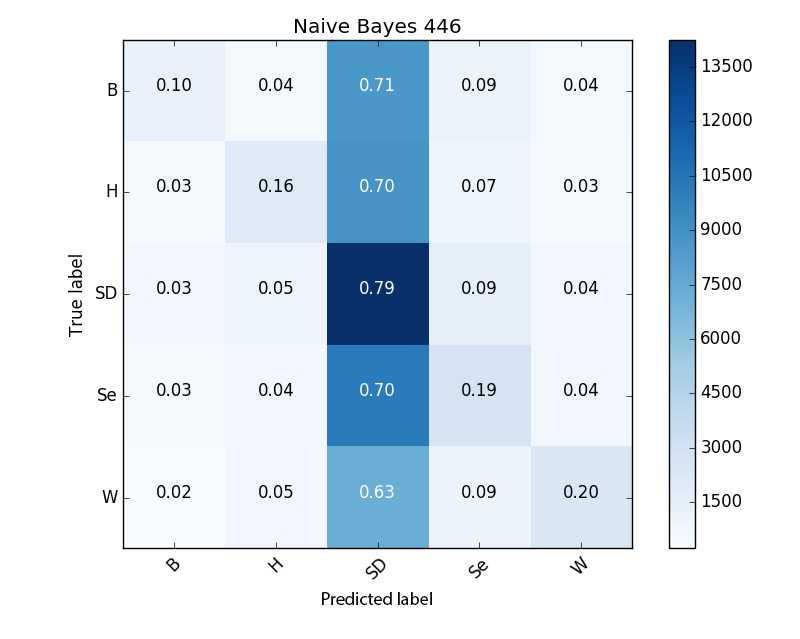
\includegraphics[width=0.5\textwidth]{confMatrixNB446Fixed}
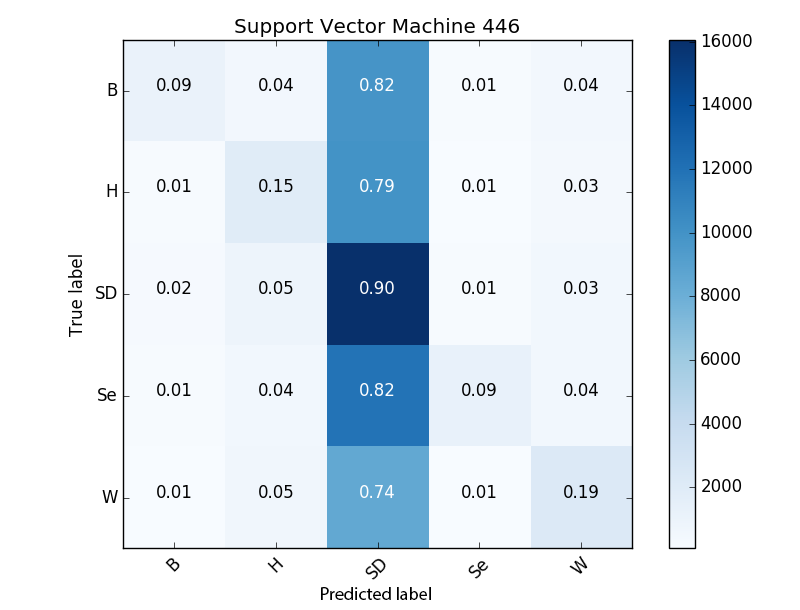
\includegraphics[width=0.5\textwidth]{confMatrixSVM446Fixed}
There are two main observations to be made about this graphic. Firstly, both of these confusion matrices demonstrate clearly the strong selection bias towards San Diego discussed earlier. Secondly, in a confusion matrix, strong top-left to bottom-right diagonals  represent good classifier performance. While difficult to tell (and both are fairly poor), Naive Bayes does appear to have a stronger general diagonal than SVM.

\section{Conclusion}
Evaluating evaluation itself is difficult, but it can be conceded that F-Score, the focus of this report, isn't perfect. There are many different ways to parameterise or average even this one metric, let alone the others available. None of the metrics considered use true negatives, in which the classifier correctly says what an instance is \textbf{not}. Specificity is such a measure, and could be interesting in further study. Methods like (AU)ROC could be interesting also; a graphical approach is attractive when demonstrating functionality of a machine learner, though often not very conclusive as seen in the confusion matrices. While it's hard to decide upon a "winner", according to the evaluation metrics and methods explored here Naive Bayes is better than SVM, considering that it ties $F_{0.5}Score$ and wins based on runtime and a visual inspection of confusion matrices. Given resources, the best way to approach evaluating a classifier is to look at \textit{all} the metrics available and consider each as they merit.

\hfill \break

\noindent Word Count: 1315 (within 10\%).

\vfill\eject
\printbibliography
\clearpage
\section{Appendices}
\subsection{Appendix 1: Results from different classifiers and data-sets}
Not all results are included here, only those referenced in the report. See allResults.txt for best35 and best446 results printouts for Naive Bayes and SVM.
\subsubsection{Zero-R Best 446}
\begin{verbatim}
     precision  recall  f0.50   support
 B   0.00       0.00    0.00    12061
 H   0.00       0.00    0.00    12578
SD   0.26       1.00    0.31    17929
Se   0.00       0.00    0.00    14482
 W   0.00       0.00    0.00    11482

avg  0.05       0.20    0.06    68532

Time taken to train the model: 4.76 sec
Time taken to test the model: 1.25 sec
\end{verbatim}
\subsubsection{Naive Bayes Best 446}
\begin{verbatim}
     precision  recall  f0.50   support
 B   0.44       0.10    0.27    12061
 H   0.44       0.16    0.33    12578
SD   0.29       0.79    0.33    17929
Se   0.37       0.19    0.31    14482
 W   0.51       0.20    0.39    11482

avg  0.41       0.29    0.33    68532

Time taken to train the model: 4.94 sec
Time taken to test the model: 6.21 sec
\end{verbatim}
\vfill\eject
\subsubsection{SVM Best 446}
\begin{verbatim}
     precision  recall  f0.50   support
 B   0.61       0.09    0.29    12061
 H   0.44       0.15    0.32    12578
SD   0.29       0.90    0.33    17929
Se   0.69       0.09    0.30    14482
 W   0.54       0.19    0.40    11482

avg  0.51       0.29    0.33    68532

Time taken to train the model: 306.32 sec
Time taken to test the model: 6.79 sec
\end{verbatim}

\subsection{Appendix 2: Short comment on topics not covered by this report}
This report is not concerned with the bias-variance trade-off, nor with feature engineering. As such, data is segmented according to the holdout method as per the given data-sets best35 and best446 \footnote{Feature selection thanks to Jeremy Nicholson}. As a shallow comment, bias will have been reduced in the 446 data-set vs. the 35 data-set due to a greater breadth of features with which instances are classified. Considering that there are potentially hundreds of thousands of features in the full data-set, a small selection such as 446 should hopefully not introduce too much variance. There is not much that can be done about noise, namely tweets in which the content is not related to the user's location. Tweets \textit{could} be grouped based on user ID to help decide on location, but this is not the objective of this report.

\end{document}